\documentclass[12pt]{report}
%% Language and font encodings
\usepackage[italian]{babel}
\usepackage[utf8x]{inputenc}
\usepackage[T1]{fontenc}
\usepackage{graphicx}
\usepackage{caption}
\usepackage{subcaption}
\usepackage[cache=false]{minted}
\usepackage[table]{xcolor}
%% Sets page size and margins
\usepackage[a4paper,top=2cm,bottom=2cm,left=2cm,right=2cm,marginparwidth=1.75cm]{geometry}
\usepackage{amssymb}
\usepackage{amsmath}
\usepackage{xcolor}
\usepackage{titlesec}
\usepackage{hyperref}
\usepackage{subfiles}
\usepackage{mathtools}
\usepackage{tcolorbox}
\usepackage{mdframed}


\titleclass{\subsubsubsection}{straight}[\subsection]
\newmdtheoremenv{theo}{Definizione}

\newcounter{subsubsubsection}[subsubsection]
\renewcommand\thesubsubsubsection{\thesubsubsection.\arabic{subsubsubsection}}
\renewcommand\theparagraph{\thesubsubsubsection.\arabic{paragraph}} % optional; useful if paragraphs are to be numbered

\titleformat{\subsubsubsection}
  {\normalfont\normalsize\bfseries}{\thesubsubsubsection}{1em}{}
\titlespacing*{\subsubsubsection}
{0pt}{3.25ex plus 1ex minus .2ex}{1.5ex plus .2ex}

\makeatletter
\renewcommand\paragraph{\@startsection{paragraph}{5}{\z@}%
  {3.25ex \@plus1ex \@minus.2ex}%
  {-1em}%
  {\normalfont\normalsize\bfseries}}
\renewcommand\subparagraph{\@startsection{subparagraph}{6}{\parindent}%
  {3.25ex \@plus1ex \@minus .2ex}%
  {-1em}%
  {\normalfont\normalsize\bfseries}}
\def\toclevel@subsubsubsection{4}
\def\toclevel@paragraph{5}
\def\toclevel@paragraph{6}
\def\l@subsubsubsection{\@dottedtocline{4}{7em}{4em}}
\def\l@paragraph{\@dottedtocline{5}{10em}{5em}}
\def\l@subparagraph{\@dottedtocline{6}{14em}{6em}}
\makeatother

\setcounter{secnumdepth}{4}
\setcounter{tocdepth}{4}


%opening
\title{Cittadinanza Digitale e Tecnocivismo \\ \large Riassunti}
\author{Andrea Pennati}
\date{}

\begin{document}

    \maketitle
    \tableofcontents
    \clearpage
    \chapter{Introduzione}
\textbf{L'Arcobaleno della Cittadinanza Digitale} è un \emph{framework} il cui scopo è quello di rappresentare gli aspetti della cittadinanza digitale in livelli concettuali. Il modello è così articolato:
\begin{itemize}
    \item I livelli più bassi definiscono le caratteristiche tecnico-infrastrutturali,
    \item I livelli più alti riguardano il diritto di un cittadino al coinvolgimento attivo nel processo decisionale.
\end{itemize}
\begin{figure}[h!]
    \centering
    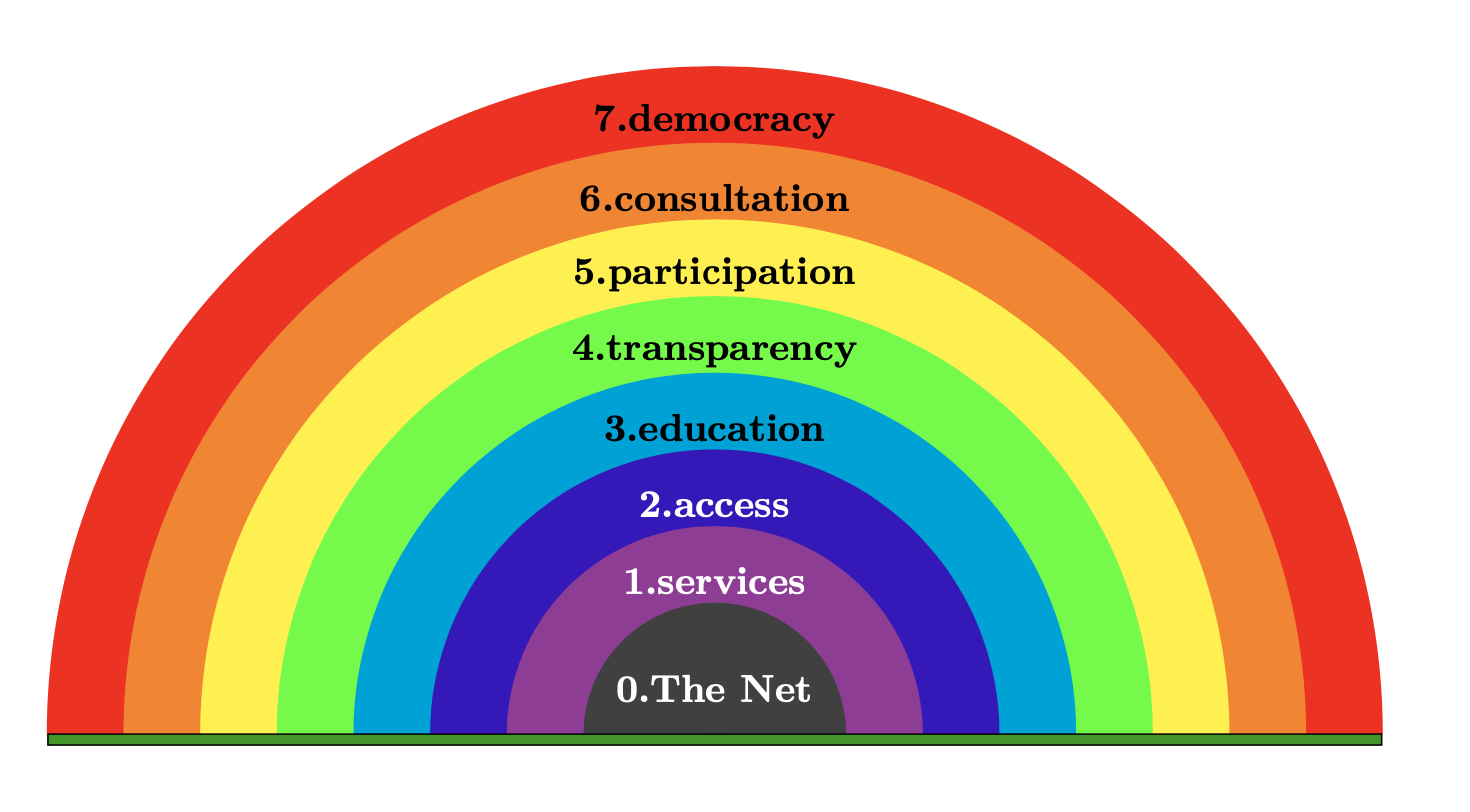
\includegraphics[scale=0.5]{img/rainbow.png}
    \caption{Arcobaleno della Cittadinanza Digitale e Tecnocivismo}
    \label{fig:rainbow}
\end{figure}

    \chapter{Livello 0 [\emph{La Rete}]}
Internet è una \textbf{rete digitale di trasporto dati} che serve a portare grosse quantità di informazioni a velocità molto elevate. Il funzionamento si basa sulla trasmissione di blocchi di dati, chiamati \textbf{pacchetti}, che vengono ordinati in sequenze che formano \textbf{flussi di dati} usufruibili dagli utenti.
\bigbreak
Uno dei princìpi della Rete che può essere associato alla Cittadinanza Digitale prende il nome di \textbf{relatività}. Preso direttamente dal mondo della Fisica, afferma che: \textbf{non possono esistere due osservatori che vedono la Rete allo stesso modo.}
Alcuni esempi possono essere:
\begin{itemize}
    \item \textbf{Domain Name System}: i provider nazionali, durante la risoluzione dei DNS di siti considerati illegali su territorio nazionale, sono obbligati a fornire indirizzi IP sbagliati in modo da non consentirne l'accesso,
    \item \textbf{Firewall}: il traffico dati viene bloccato a seconda della tipologia di protocollo utilizzato. Un esempio significativo è rappresentato dal \emph{Great Firewall} cinese\footnote{\url{https://it.wikipedia.org/wiki/Great_Firewall}},
    \item \textbf{Velocità}: i provider possono applicare una specifica tariffa a seconda della velocità del traffico della rete privilegiando gli utenti che sono disposti a pagare di più,
\end{itemize}
\bigbreak
Oggigiorno le tecnologie permettono la \textbf{memorizzazione di grandi quantità di dati} per tempi pressoché infiniti. Da diversi anni multinazionali e governi, con la scusa della lotta al terrorismo, sono riusciti ad allungare a dismisura i \textbf{tempi di conservazione dei dati raccolti}.
\bigbreak
L'incredibile valore che hanno assunto i dati nel corso del XXI secolo è dettato dalle innumerevoli forme di utilizzo, come:
\begin{itemize}
    \item \textbf{Personalizzazione dei servizi}: profilare gli utenti consente alle aziende di offrire un servizio su misura per ogni utente,
    \item \textbf{Analisi di mercato}: i dati possono essere analizzati anticipando le nuove esigenze di mercato,
    \item \textbf{Manipolazioni politiche}: è possibile mostrare agli utenti contenuti \emph{ad hoc} in modo da influenzare le loro convinzioni politiche,
\end{itemize}

\bigbreak
Purtroppo Internet è stata progettata da "\emph{ingenui}"; coloro che hanno creato questa rete non ne hanno immaginato un uso così \textbf{distorto}.
La maggior parte dei \textbf{protocolli di comunicazione} sicura, vale a dire crittografata, utilizzati su Internet basano la propria sicurezza su \textbf{certificati crittografici a chiave pubblica} emessi secondo lo standard X.509 e gestiti per mezzo di una \emph{PKI} globale.
In generale questo tipo di architettura è debole in quanto costringe i fruitori del servizio a fidarsi incondizionatamente delle organizzazione che rilasciano tali certificati.

Una possibile soluzione sarebbe stata quella di progettare il protocollo IP includendo sin da subito l'utilizzo della crittografia, ma tale idea fu abbandonata a causa delle pressioni esercitate dal governo statunitense.
\bigbreak
GNUnet\footnote{\url{https://www.gnunet.org/en/}} è uno stack di protocolli di rete per la creazione di applicazioni sicure, distribuite e che preservano la privacy, il cui obiettivo è quello di sostituire il vecchio stack di protocolli dell'attuale Internet.

Questa tecnologia si basa sul fatto che  ogni nodo si connette direttamente con il maggior numero di altri nodi e collabora per instradare efficientemente i pacchetti, \textbf{senza che sia necessario conoscere la destinazione finale o il contenuto dei pacchetti stessi, metadati compresi}.
    \chapter{Livello 1 [\emph{services}]}
La disponibilità di servizi online che rispecchiano quelli fisici, può avere un impatto significativo sui diritti di cittadinanza, soprattutto per quelli erogati dalla \textbf{Pubblica Amministrazione}.
\bigbreak
Con il termine \textbf{digitalizzazione dei servizi} si indica il processo attraverso cui un servizio, originariamente erogato in forma analogica, viene implementato e distribuito attraverso l'utilizzo di tecnologie digitali. I servizi digitali offrono vantaggi quali scalabilità e velocità, ma non offrono altrettante garanzie in termini di flessibilità. 

Per arginare questo problema è necessario non effettuare una totale migrazione in favore del digitale ma mantenere una parte del servizio in forma analogica; è fondamentale avere un meccanismo di \textbf{fallback}.
\bigbreak
L'\textbf{interoperabilità} offre innumerevoli vantaggi perché permette agli utenti  di migrare da un sistema all'altro in maniera efficace e semplice. Per rendere questa procedura realizzabile è necessario che i protocolli e il formato dei dati siano sempre gli stessi.

Se da una parte i benefici lato utente sono evidenti, dall'altra le aziende mirano ad utilizzare protocolli e formati proprietari in modo da ottenere un rapporto di dipendenza che prende il nome di \textbf{vendor lock-in}\footnote{\url{https://it.wikipedia.org/wiki/Vendor_lock-in}}. Sempre più spesso le aziende credono che la possibilità che un utente possa cambiare sistema sia un male; poiché potrebbero vedere una grossa fetta di utenza migrare verso sistemi migliori.
\bigbreak
Uno dei \textbf{vantaggi} principali dei servizi digitali è rappresentato dalla possibilità di avere un sistema estremamente scalabile. L'avvento delle \textbf{Server Farm}\footnote{\url{https://it.wikipedia.org/wiki/Server_farm}} ha permesso l'allocazione "illimitata" di risorse.
\bigbreak
Un servizio digitale deve garantire che, durante l'interazione con un utente, la raccolta e la \textbf{conservazione dei dati avvenga in maniera sicura per proteggere la privacy}. 
Garantire la privacy è un problema molto importante perché l'interazione tra utente e servizio digitale lascia \textbf{tracce importanti, indistruttibili e spesso associabili a una singola persona}\footnote{Principio di Locard \emph{digitale} della Rete: un'informazione immessa nella Rete:\begin{itemize}
    \item lascia sempre tracce,
    \item tutt'altro che esigue,
    \item indistruttibili.
\end{itemize}}.

\bigbreak
Ogni servizio digitale deve essere più inclusivo possibile; ci si deve preoccupare di \textbf{non escludere utenti con abilità fisiche limitate}. 

A tal proposito esistono alcune normative che nel corso del tempo hanno portato alle linee guida attuali per la realizzazione di siti web della Pubblica Amministrazione \textbf{accessibili}, che fino al 2014 lo erano ancora poco.
\bigbreak
I servizi sono relativistici: non possono esistere due osservatori che vedono un servizio allo stesso modo. Esistono diversi casi in cui si manifesta questa situazione di relatività:
\begin{itemize}
    \item \textbf{Price discrimination}: strategia commerciale che impone a consumatori diversi, prezzi diversi per l’acquisto dello stesso bene offerto, a seconda delle caratteristiche conosciute,
    \item \textbf{Contenuti personalizzati}: Social Media e diversi motori di ricerca mostrano contenuti personalizzati a seconda della conoscenza che hanno di un utente.
\end{itemize}
    \chapter{Livello 2 [\emph{access}]}
Nel livello 2 vengono analizzati i servizi pubblici base a cui un cittadino deve avere accesso e le relative problematiche di accesso. Un servizio pubblico deve essere strutturato in modo tale da poterne usufruire in maniera \textbf{indiscriminata}; deve mirare a soddisfare le necessità e il suo costo deve essere distribuito sull'intera collettività. Un servizio riconosciuto legislativamente deve essere erogato in linea con i principi di continuità, doverosità, parità di trattamento, economicità e possibilità di connessione; questi aspetti rappresentano quello che viene definito \textbf{Service Level Agreement}.
Una nazione civile deve offrire ai suoi cittadini \textbf{servizi di base} che permettano di vivere, muoversi, istruirsi, lavorare, socializzare, realizzarsi, ecc. Maslow ha ideato una \textbf{gerarchia di bisogni umani} in cui ogni livello descrive una lista di necessità. 

I servizi che si occupano di soddisfare questi bisogni primari sono chiari, ma per un per un cittadino \textbf{digitale} quali dovrebbero essere i servizi essenziali?
\bigbreak
Un servizio diventa pubblico quando viene legislativamente riconosciuto come tale. Ogni servizio pubblico deve essere erogato secondo questi principi:
\begin{itemize}
    \item \textbf{Doverosità}: lo Stato si fa carico di garantire l’erogazione del servizio,
    \item \textbf{Continuità}: il servizio deve essere garantito in maniera continuativa,
    \item \textbf{Parità di trattamento}: l’accesso ai servizi deve essere  equo per tutti i cittadini,
    \item \textbf{Universalità}: i servizi devono essere garantiti senza alcun tipo di discriminazione,
    \item \textbf{Economicità}: il gestore del servizio deve conseguire un margine ragionevole di utile,
    \item \textbf{Possibilità di concessione}: lo Stato può concedere l’erogazione di alcuni servizi a enti esterni a patto che ne garantisca l'accesso e la qualità.
\end{itemize}

\bigbreak
Lo Stato deve garantire a tutti i cittadini che i servizi, analogici o digitali che siano, siano concessi in maniera indiscriminata. 

Il fenomeno del \textbf{digital divide} misura le disuguaglianze nella disponibilità di accesso alle tecnologie digitali da parte della popolazione. In Italia, nonostante non sia uno dei paesi peggiori da questo punto di vista, questa \textbf{disuguaglianza} è presente soprattutto se si paragonano le infrastrutture del Nord Italia con quelle del Sud Italia.

\bigbreak
Per cercare di colmare questo divario tecnologico lo Stato dovrebbe concentrare le proprie risorse in modo da avere una \textbf{copertura adeguata del cablaggio della fibra ottica}. Una buona copertura avrebbe un impatto positivo immediato: garantirebbe maggiore produttività a livello imprenditoriale e un’istruzione più efficiente.

Un altro aspetto importante potrebbe essere quello di offrire ai cittadini un \textbf{sistema di archiviazione basato su cloud} per facilitare l'archiviazione di documenti legati alla Pubblica Amministrazione.

Infine sembra ragionevole pensare che ogni cittadino debba possedere un \textbf{indirizzo di posta elettronica ufficiale} in modo da semplificare la comunicazione con la Pubblica Amministrazione. Per ogni servizio digitale dovrebbe essere creato un account verificato per potervi accedere; a tal proposito in Italia è stato implementato il \textbf{Sistema Pubblico di Identità Digitale}, meglio noto come SPID, che permette l'accesso controllato a quasi tutti i servizi della Pubblica Amministrazione.

\bigbreak
Nel mondo esistono movimenti, come la \textbf{Net Neutrality}, che si battono per cercare di eliminare la \textbf{relatività} imposta dagli \textbf{Internet Service Provider (ISP)}, che dovrebbero essere trasparenti e trattare qualsiasi tipo di contenuto o cittadino in modo equo e non discriminatorio.



    \chapter{Livello 3 [\emph{education}]}
Nel livello 3 vengono analizzate le problematiche e le minacce relative alla scarsa \textbf{educazione digitale}.
 Lo sviluppo tecnologico ha fatto si che i dispositivi che ci circondano siano sempre più intelligenti e pervasivi. Questa situazione ha \textbf{migliorato} la qualità della vita, ma ha reso i dispositivi più difficili da utilizzare e complessi da capire. 

Per un \textbf{cittadino digitale} è indispensabile saper conoscere, configurare e controllare i dispositivi che lo circondano in modo da non rimanerne "sopraffatto".
Nonostante esistano molti \textbf{software open source} che possono essere studiati a fondo mediante lettura del codice sorgente talvolta anch'essi sono di difficile comprensione.
\bigbreak
Molte leggi vanno controcorrente rispetto al \textbf{principio di trasparenza e comprensibilità} dei prodotti; un caso particolare riguarda l'utilizzo dei \textbf{brevetti} che limitano fortemente la conoscenza e la ricerca.
Alcune proposte di legge mirano ad eliminare o indebolire l'utilizzo della crittografia mediante l'utilizzo di una chiave "\emph{passe-partout}"\footnote{\url{https://www.treccani.it/vocabolario/passe-partout/}} utilizzabile direttamente dal governo. Utilizzano la scusa della lotta al terrorismo per mascherare le vere ragioni di questa scelta. Questa soluzione presenta delle lacune evidenti:
\begin{itemize}
    \item i criminali continuerebbero a "nascondersi" continuando le attività illegali,
    \item \textbf{i cittadini perderebbero il controllo rispetto ai propri dati e il concetto di privacy subirebbe un deciso ridimensionamento}.
\end{itemize}

Di fondamentale importanza rimane il concetto che ogni cittadino dovrebbe comprendere le tecnologie in modo da non dover delegare le scelte politiche potendo quindi partecipare attivamente nelle questioni tecnologiche.
\bigbreak
Una possibile soluzione potrebbe essere quella di sviluppare un \textbf{insegnamento orientato alla critica verso il mondo digitale}, ovvero quello che viene definito \textbf{learn to code}; poiché queste problematiche sono spesso figlie della scarsa \textbf{educazione al mondo digitale} talvolta causate dalla mancanza di volontà/possibilità del cittadino alla scoperta e all'assenza di strumenti tecnologici adatti.
\bigbreak
Un ruolo interessante viene ricoperto dai \textbf{movimenti che partono dal "basso"} e che prendono il nome di \textbf{grassroots}. Grassroots è un termine anglosassone che indica quei movimenti politici che nascono dall'aggregazione spontanea di gruppi di cittadini. L'idea nasce dal desiderio di organizzarsi autonomamente in modo da ottemperare a quelle mancanze istituzionali spesso causate dalla lontananza dal problema da parte dello Stato, oppure perché in disaccordo con ideologie non più condivisibili.
Il \textbf{Software Libero} fa parte di questi movimenti e denuncia la \textbf{necessità di concedere i diritti invece che toglierli a chi usa il software}. L'ideale sarebbe quello di avere software utilizzabili per qualsiasi scopo, \textbf{che sia possibile redistribuire e di cui si possa studiare il funzionamento}.
\bigbreak
Infine, nonostante le leggi siano spesso lo strumento del "male", queste possono essere sfruttate in maniera positiva. Esistono delle iniziative, che prendono il nome di \textbf{"right to repair"}, che fanno pressione sui governi affinché questi emanino delle leggi che costringano i produttori di dispositivi elettronici a \textbf{renderli facilmente riparabili} dagli utenti in maniera autonoma.



    \chapter{Livello 4 [\emph{transparency}]}
Il livello 4  tratta della problematica della trasparenza ed è il primo livello in cui si analizza il rapporto di comunicazione tra Istituzioni e cittadino.
Nel contesto "Cittadinanza Digitale e Tecnocivismo" si parla di \textbf{trasparenza} applicandola sia ai sistemi digitali sia ai sistemi organizzativi, che per essere trasparenti devono \textbf{rendere pubbliche} informazioni sul proprio stato interno. In particolare quando si parla di relazione tra Pubblica Amministrazione e cittadino si ha un tipo di \textbf{trasparenza "top-down"}, ovvero fatta da un ente che svolge un \textbf{servizio pubblico} verso il cittadino.
\bigbreak
La Pubblica Amministrazione rimane sempre contraria nell'essere trasparente verso i cittadini. Dare ad un cittadino la possibilità di accedere a dati oggettivi \textbf{permetterebbe a quest'ultimo di acquisire consapevolezza rispetto all'utilizzo delle risorse pubbliche e alle decisioni prese per la comunità}.

Un cittadino ha molta più \textbf{fiducia} nei confronti di un \textbf{ente trasparente}, mentre resterà restio nel credere nella bontà di quest'ultimo se non sarà trasparente rispetto al proprio operato.
\bigbreak
La struttura attraverso cui la Pubblica Amministrazione pubblica i dati in suo possesso prende il nome di \textbf{Open Data}. Purtroppo \textbf{non esiste uno standard} che uniforma le modalità attraverso cui i dati devono essere pubblicati; questo implica che la maggior parte delle volte i dati sono:
\begin{itemize}
    \item \textbf{rilasciati con un formato chiuso},
    \item \textbf{inutili},
    \item \textbf{illeggibili}.
\end{itemize}
\bigbreak
Una possibile soluzione è stata proposta da Tim Berners-Lee che si basa sull'assegnamento di un punteggio che può variare a seconda dell'\textbf{esistenza del dato, dal fatto che sia leggibile, che possieda un formato libero e che sia connesso ad altri dati con standard} \textbf{Resource Description Framework (RDF)}\footnote{\url{https://it.wikipedia.org/wiki/Resource_Description_Framework}}. 
Questo tipo di valutazione mitiga il problema da un punto di vista informatico, ma non tratta aspetti importanti come la licenza, l'aggiornamento e l'utilità.

Davies, a tal proposito, ha definito una valutazione che prende in considerazione l'utilità dei dati, il contesto, la discussione rispetto a quest'ultimi e la possibilità di integrare o modificare i dati da parte del cittadino.

\bigbreak
Queste soluzioni vanno a scontrarsi con gli\textbf{ “Webstacles”}; ovvero gli ostacoli che mettono in atto le P.A. per fare in modo che i dati non siano modificabili dall’utente finale, quindi si hanno informazioni rilasciate con formati particolari per evitare che un utente terzo possa fare qualsiasi tipo di operazione, risultando, “legalmente” trasparente, ma essendolo relativamente poco nella pratica.
Capita che i \textbf{dati vengano pubblicati in maniera frammentata}, oppure mediante l'inserimento di un \textbf{captcha} per ogni download.

Alcune soluzioni, come lo \textbf{scraping}, prevedono l'estrazione dei dati grezzi e la conseguente aggregazione ai fini di rendere le informazioni disponibili in maniera compatta e comprensibile.
Nel caso in cui i dati non siano stati pubblicati \textbf{è possibile tentarne una ricostruzione mediante la raccolta sul campo} piuttosto che attraverso l'estrazione da qualche dataset.
\bigbreak
Da un punto di vista legislativo è doveroso menzionare il \textbf{Freedom of Information Act (FOIA)} che in linea teorica darebbe il potere ai cittadini di chiedere qualsiasi informazione riguardante la Pubblica Amministrazione.

\end{document}